% skyrius apie matematinį modelį

\section{Matematinis modelis}

\subsection{Bedimensis modelis}

\begin{subequations} \label{nodim}
    \begin{align}
    \frac{\partial c_1}{\partial t}&=-3c_1c_2+D\Delta c_1 \label{nodim1}\\
    \frac{\partial c_2}{\partial t}&=-5c_1c_2+D\Delta c_2 \label{nodim2}\\
    \frac{\partial c_3}{\partial t}&=2c_1c_2
    \end{align}
\end{subequations}

kur $c_1,c_2,c_3$ yra bedimensė medžiagų koncentracija, 
$\Delta$ - Laplaso operatorius, $t$ - laikas, 
$D$ - bedimensis medžiagų $c_1$ ir $c_2$ difuzijos koeficientas. Modeliui yra taikoma kraštinė sąlygą:

\begin{equation} \label{general-boundary-cond}
  \nabla c_k(\textbf{x}, t)\cdot\vec{n}=0, \textbf{x}\in\partial\Omega
\end{equation}

Čia $\nabla c_k$ yra medžiagos $c_k$ gradientas, $\textbf{x}$ - erdvės koordinatė, $\partial\Omega$ - simuliuojamos erdvės srities paviršius, o $\vec{n}$ - simuliuojamos erdvės paviršiaus normalė.

\subsection{Elementų maišymasis dviejose dimensijose}

Interpretavus bedimensį modelį \eqref{nodim} dviejose dimensijose gauname lygtis

\begin{subequations} \label{rect}
    \begin{align}
    \frac{\partial c_1}{\partial t}&=-3c_1c_2+D\left(\frac{\partial^2c_1}{\partial x^2}+\frac{\partial^2c_1}{\partial y^2}\right)\\
    \frac{\partial c_2}{\partial t}&=-5c_1c_2+D\left(\frac{\partial^2c_2}{\partial x^2}+\frac{\partial^2c_2}{\partial y^2}\right)\\
    \frac{\partial c_3}{\partial t}&=2c_1c_2
    \end{align}
\end{subequations}

\newpage
Šiam modeliui yra taikomos stoichiometrinės pradinės sąlygos:

% pradinės sąlygos medžiagų koncentracijai turėtų aprašyti stoichiometrinį mišinį

\begin{equation} \label{intial-cond}
  \begin{aligned}
  c_1(x, y, 0) &= \begin{cases} 3c_0, & \text{jei } x \in A \\ 0, & \text{kitaip} \end{cases}\\
  c_2(x, y, 0) &= \begin{cases} 5c_0, & \text{jei } x \notin A \\ 0, & \text{kitaip} \end{cases}\\
  c_3(x, y, 0) &= 0,\\ 
  (x, y) &\in \Omega, \quad\Omega=[0,W]\times[0,H],\quad A=\left[0,\tfrac{W}{2}\right]\times\left[0,\tfrac{H}{2}\right] \cup \left[\tfrac{W}{2},W\right]\times\left[\tfrac{H}{2},H\right].
\end{aligned}
\end{equation}

Čia $c_0$ yra kažkoks teigiamas dydis, kuris nusako pradinę kiekvienos medžiagos koncentraciją sistemoje.

\begin{figure}[h!]
  \centering
  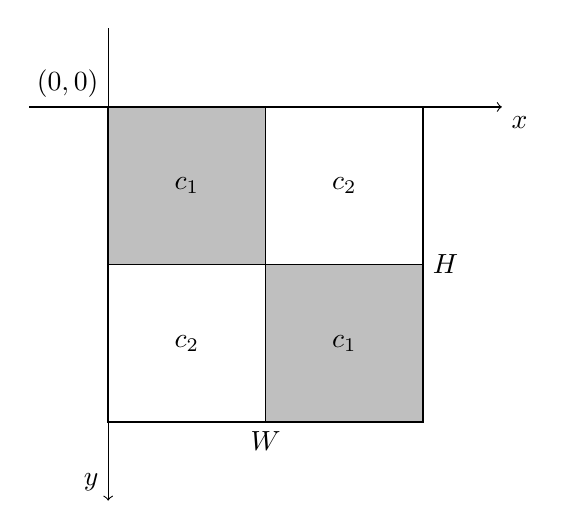
\begin{tikzpicture}[scale=2.0]
      \draw[fill=white] (0,0) rectangle (1,1);
      \draw[fill=white] (1,1) rectangle (2,2);
      \draw[fill=gray!50] (0,1) rectangle (1,2);
      \draw[fill=gray!50] (1,0) rectangle (2,1);
      
      % Draw the boundary of the square
      \draw[thick] (0,0) rectangle (2,2);
  
      % Draw axes
      \draw[->] (-0.5,2) -- (2.5,2) node[anchor=north west] {$x$};  % x-axis
      \draw[<-] (0,-0.5) node[anchor=south east] {$y$} -- (0,2.5);  % y-axis
  
      % Mark the origin
      \node[anchor=south east] at (0,2) {$(0, 0)$};
      
      % Mark the side length L
      \draw[-] (2,0) -- (2,2) node[midway, right] {$H$};
      \draw[-] (0,0) -- (2,0) node[midway, below] {$W$};
      \draw (0.5, 1.5) node[anchor=center] {$c_1$};
      \draw (1.5, 0.5) node[anchor=center] {$c_1$};
      \draw (1.5, 1.5) node[anchor=center] {$c_2$};
      \draw (0.5, 0.5) node[anchor=center] {$c_2$};
  \end{tikzpicture}
  \caption{Sistemos pradinės sąlygos}
\end{figure}

kraštinės sąlygos \eqref{general-boundary-cond} dviejose dimensijose virsta:

\begin{equation} \label{boundary-cond}
\begin{split}
\frac{\partial c_1}{\partial x}\Big|_{x=0}&=\frac{\partial c_1}{\partial x}\Big|_{x=L}=\frac{\partial c_2}{\partial x}\Big|_{x=0}=\frac{\partial c_2}{\partial x}\Big|_{x=L}=0, \quad y\in[0,H], \quad t\in[0,T]\\
\frac{\partial c_1}{\partial y}\Big|_{y=0}&=\frac{\partial c_1}{\partial y}\Big|_{y=L}=\frac{\partial c_2}{\partial y}\Big|_{y=0}=\frac{\partial c_2}{\partial y}\Big|_{y=L}=0, \quad x\in[0,W],\quad t\in[0,T]
\end{split}
\end{equation}

kur $L$ - bedimensis kubo kraštinės ilgis, $T$ - bedimensė proceso trukmė.

\section{Skaitinis modelis}

\subsection{Erdvės diskretizavimas Dekarto koordinačių sistemoje}

Dviejų dimensijų skaitiniam modeliui erdvė buvo padalinta į $N \times M$ taškų 
nutolusių vienas nuo kito fiksuotais $\Delta x$ ir $\Delta y$ atstumais.

\begin{figure}[!h]
\centering
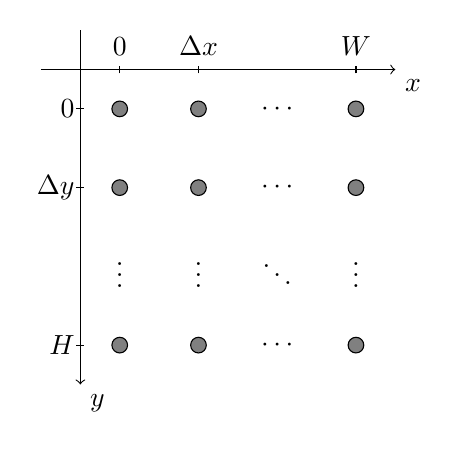
\begin{tikzpicture}

   % Set up styles for the grid
  \tikzset{
    node/.style={circle, draw, fill=gray, inner sep=2pt},
    ellipsis/.style={draw=none, fill=none}
  }

  \draw[->] (0, -0.5) -- (4.5, -0.5) node[anchor=north west] {$x$};  % x-axis
  % x-axis ticks
  \draw[-] (1, -0.55) -- (1, -0.45) node[anchor=south] {$0$};
  \draw[-] (2, -0.55) -- (2, -0.45) node[anchor=south] {$\Delta x$};
  \draw[-] (4, -0.55) -- (4, -0.45) node[anchor=south] {$W$};
  
  \draw[<-] (0.5,-4.5) node[anchor=north west] {$y$} -- (0.5, 0);  % y-axis
  % y-axis ticks
  \draw[-] (0.45, -1) -- (0.55, -1) node[anchor=east] {$0$};
  \draw[-] (0.45, -2) -- (0.55, -2) node[anchor=east] {$\Delta y$};
  \draw[-] (0.45, -4) -- (0.55, -4) node[anchor=east] {$H$};


  % Draw the 3x3 grid of colored circles in a 4x4 layout
  \foreach \x in {1, 2, 4} {
    \foreach \y in {1, 2, 4} {
      \node[node] at (\x, -\y) {};
    }
  }

  % Add ellipses in the 4th row and column for continuation

  \node[ellipsis] at (3, -1) {$\cdots$};
  \node[ellipsis] at (3, -2) {$\cdots$};
  \node[ellipsis] at (3, -4) {$\cdots$};

  \node[ellipsis] at (1, -3) {$\vdots$};
  \node[ellipsis] at (2, -3) {$\vdots$};
  \node[ellipsis] at (4, -3) {$\vdots$};

  \node[ellipsis] at (3, -3) {$\ddots$};

\end{tikzpicture}
\caption{ diskretizuota erdvė }
\end{figure}

Čia 

\subsection{Dviejų dimensijų skaitinis modelis Dekarto koordinačių sistemoje}

Remiantis išreikštiniu baigtinių skirtumų metodu iš dvimačio modelio galima gauti skaitinį modelį.
\begin{subequations} \label{numerical-eqs}
\begin{align}
\frac{c^{n+1}_{1,i,j}-c^n_{1,i,j}}{\Delta t}&=
-3c^{n}_{1,i,j}c^{n}_{2,i,j}\notag\\
&+D\left(\frac{c^n_{1,i-1,j}-2c^n_{1,i,j}+c^n_{1,i+1,j}}{(\Delta x)^2}+\frac{c^n_{1,i,j-1}-2c^n_{1,i,j}+c^n_{1,i,j+1}}{(\Delta y)^2}\right)\\
\frac{c^{n+1}_{2,i,j}-c^n_{2,i,j}}{\Delta t}&=
-5c^{n}_{1,i,j}c^{n}_{2,i,j}\notag\\
&+D\left(\frac{c^n_{2,i-1,j}-2c^n_{2,i,j}+c^n_{2,i+1,j}}{(\Delta x)^2}+\frac{c^n_{2,i,j-1}-2c^n_{2,i,j}+c^n_{2,i,j+1}}{(\Delta y)^2}\right)\\
\frac{c^{n+1}_{3,i,j}-c^n_{3,i,j}}{\Delta t}&=2c^{n}_{1,i,j}c^{n}_{2,i,j},
\end{align}
\end{subequations}

kur $n\in[0, T)$ - laiko momentas, 
$i\in[0,N)$ - diskrečios erdvės taško koordinatė $x$ ašyje,
$j\in[0,M)$ - diskrečios erdvės taško koordinatė $y$ ašyje,
$c^n_{1,i,j}$ - pirmos medžiagos kiekis diskrečios erdvės taške $i$, $j$ laiko momentu $n$,
$c^n_{2,i,j}$ - antros medžiagos kiekis diskrečios erdvės taške $i$, $j$ laiko momentu $n$,
$c^n_{3,i,j}$ - trečios medžiagos kiekis diskrečios erdvės taške $i$, $j$ laiko momentu $n$,
$\Delta t$ - laiko žingsnis,
$\Delta x$ - diskrečios erdvės žingsnis $x$ ašimi,
$\Delta y$ - diskrečios erdvės žingsnis $y$ ašimi.